\documentclass[12pt,a4paper,oneside]{report}

\usepackage{units}
\usepackage{numprint}

% margins
\usepackage{vmargin}
\setmarginsrb{25mm}{15mm}{25mm}{15mm}{0mm}{0mm}{0mm}{0mm}

\usepackage{tikz}
\usepackage{pgfmath}
\usetikzlibrary{scopes}
\usetikzlibrary{calc}

\begin{document}
\thispagestyle{empty}

\null\hfil{\bf\huge Faderbox - Wire Sheet}

\def\wireblock#1#2#3{
	\vfil
	\nprounddigits{2}
	\begin{tikzpicture}
		\pgfmathsetmacro{\LenghtInInch}{#2 * 2.54}
		\draw node [above right] {#1x $\unit[\numprint{#2}]{cm}$ ($\unit[\numprint{\LenghtInInch}]{in}$): #3 wire};
		\path (0,0) coordinate (a) (#2cm,0) coordinate (b);
		\draw ($ (a) + (-5mm,0) $) -- ($ (b) + (+5mm,0) $);
		\draw ($ (a) + (0,-1mm) $) -- ($ (a) + (0,+1mm) $);
		\draw ($ (b) + (0,-1mm) $) -- ($ (b) + (0,+1mm) $);
	\end{tikzpicture}
}

\vbox to 0px{
\vskip3em
\hfill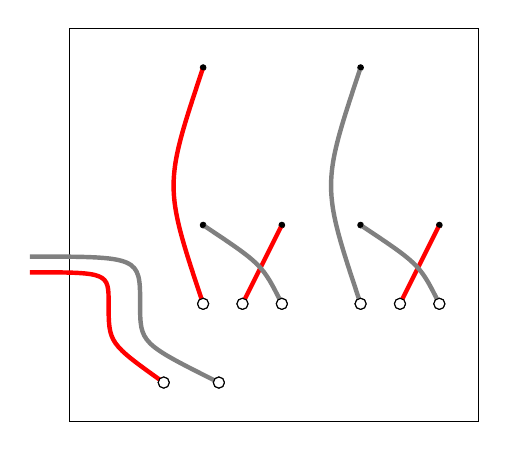
\begin{tikzpicture}

	\draw (-1.7,-2.5) rectangle (3.5,2.5);

	\draw (0,0) coordinate (l3) circle (1pt);
	\draw (1,0) coordinate (l2) circle (1pt);
	\draw (0,2) coordinate (l1) circle (1pt);

	\draw (2,0) coordinate (r3) circle (1pt);
	\draw (3,0) coordinate (r2) circle (1pt);
	\draw (2,2) coordinate (r1) circle (1pt);

	\draw (0.0,-1) coordinate (L1) circle (2pt);
	\draw (0.5,-1) coordinate (L2) circle (2pt);
	\draw (1.0,-1) coordinate (L3) circle (2pt);

	\draw (2.0,-1) coordinate (R1) circle (2pt);
	\draw (2.5,-1) coordinate (R2) circle (2pt);
	\draw (3.0,-1) coordinate (R3) circle (2pt);

	\draw (-0.5,-2) coordinate (X1) circle (2pt);
	\draw (+0.2,-2) coordinate (X2) circle (2pt);

	\draw[red,ultra thick] (l1) .. controls ++(-0.5,-1.5) .. (L1);
	\draw[gray,ultra thick] (r1) .. controls ++(-0.5,-1.5) .. (R1);

	\draw[red,ultra thick] (l2) -- coordinate (a) (L2);
	\draw[red,ultra thick] (r2) -- coordinate (b) (R2);

	\draw[gray,ultra thick] (l3) .. controls (a) .. (L3);
	\draw[gray,ultra thick] (r3) .. controls (b) .. (R3);

	\draw[red,ultra thick] (X1) .. controls ++(-0.7,0.5) .. ++(-0.7,1) .. controls ++(0,0.4) .. ++(-1.0,0.4);
	\draw[gray,ultra thick] (X2) .. controls ++(-1,0.5) .. ++(-1,1) .. controls ++(0,0.6) .. ++(-1.4,0.6);

	\fill (l3) circle (1pt) (l2) circle (1pt) (l1) circle (1pt);
	\fill (r3) circle (1pt) (r2) circle (1pt) (r1) circle (1pt);

	\draw[fill=white] (L1) circle (2pt) (L2) circle (2pt) (L3) circle (2pt);
	\draw[fill=white] (R1) circle (2pt) (R2) circle (2pt) (R3) circle (2pt);

	\draw[fill=white] (X1) circle (2pt);
	\draw[fill=white] (X2) circle (2pt);

\end{tikzpicture}\vss
}

\wireblock{12}{2}{red}
\wireblock{12}{2}{black}

\wireblock{6}{9}{red}
\wireblock{6}{9}{black}

\wireblock{2}{4.5}{1 red and 1 black}
\wireblock{2}{6.3}{1 red and 1 black}
\wireblock{2}{8.0}{1 red and 1 black}
\wireblock{2}{9.8}{1 red and 1 black}
\wireblock{2}{11.5}{1 red and 1 black}
\wireblock{2}{13.3}{1 red and 1 black}

\end{document}

